\chapter{Czujnik ciśnienia atmosferycznego BMP085}
\section*{Opis}
Czujnik ten jest wysoce precyzyjnym, cyfrowym czujnikiem ciśnienia oraz temperatury powietrza. Jego energooszczędność oraz niskie zapotrzebowanie na zasilanie napięciem (do 3,6 V) sprawia, że jest idealnym rozwiązaniem do zastosowań w urządzeniach mobilnych codziennego użytku, tak jak telefony komórkowe, nawigacje GPS itd. Dzięki bardzo szybkiemu czasu przetwarzania danych (do 7,5 ms) oraz niskiemu wpływowi zakłóceń daje rezultaty, niewiele różniące się od warunków mierzonych.


BMP085 jest często używany w prognozowaniu pogody, ze względu na obecność dwóch czujników (ciśnienia i temperatury). Można go również wykorzystać do wyznaczenia wysokości względnej oraz bezwzględnej od poziomu morza. W tym celu używane jest prawo zależności wysokości od ciśnienia, tzw. wzór barometryczny. Po uproszczeniu wygląda on następująco:
$$ wysokosc = 44330 * (1- (\frac{p}{p_{0}})^{\frac{1}{5,255}}) $$
p - ciśnienie na badanej wysokości\newline
$ p_{0} $ - ciśnienie na poziomie odniesienia
\newline

Znając wartość ciśnienia na poziomie odniesienia, istnieje możliwość wyznaczenia względnej wysokości ciała do wysokości bazowej. Taka własność ciśnienia jest używana na lotniskach, samolot w momencie lądowania jest informowany o ciśnieniu panującym na lotnisku, piloci znają również ciśnienia panujące wokół samolotu. Na tej podstawie wyznaczana jest względna wysokość maszyny od poziomu pasa startowego.

\section*{Dane charakterystyczne}
Czujnik BMP085, zgodnie ze specyfikacją, może pracować bezpiecznie w przedziale temperatur od -40 do +85 $^\circ$C. Rozdzielczość pomiarów dla ciśnienia atmosferycznego wynosi 0.01 hPa, natomiast dla temperatury jest to 0.1 $^\circ$C. Dokładność badania ciśnienia to maksymalnie +- 4 hPa, dla temperatury to +- 2$^\circ$C.

Zdjęcia \ref{fig:bmp085_dol} oraz \ref{fig:bmp085_gora} prezentują wygląd czujnika wbudowanym w gotowy układ, z wyprowadzonymi złączami do komunikacji z mikrokontrolerami. Taki moduł został wykorzystany w projekcie inżynierskim.
\begin{figure}[h]
\centering
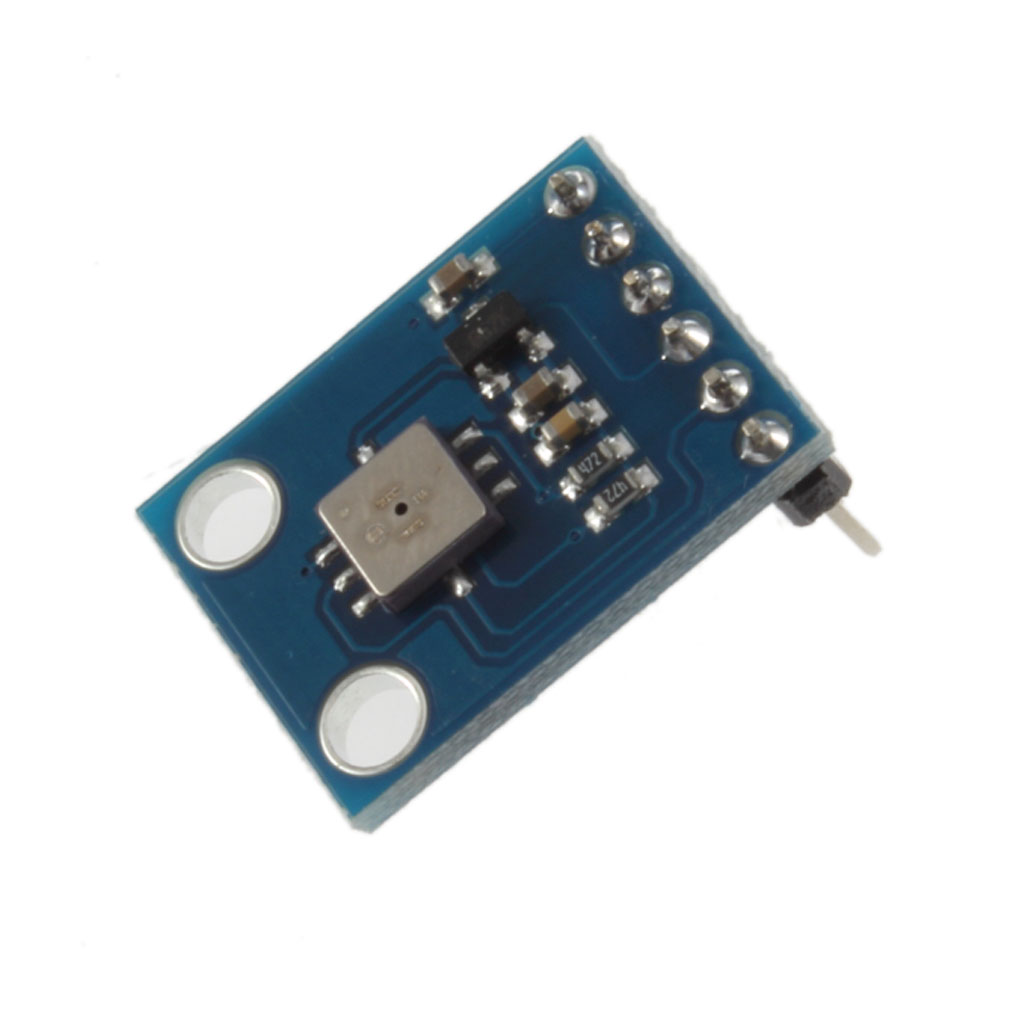
\includegraphics{bmp085_dol}
\caption{Czujnik ciśnienia BMP085 - widok z dołu}
\label{fig:bmp085_dol}
\end{figure}
\begin{figure}[h]
\centering
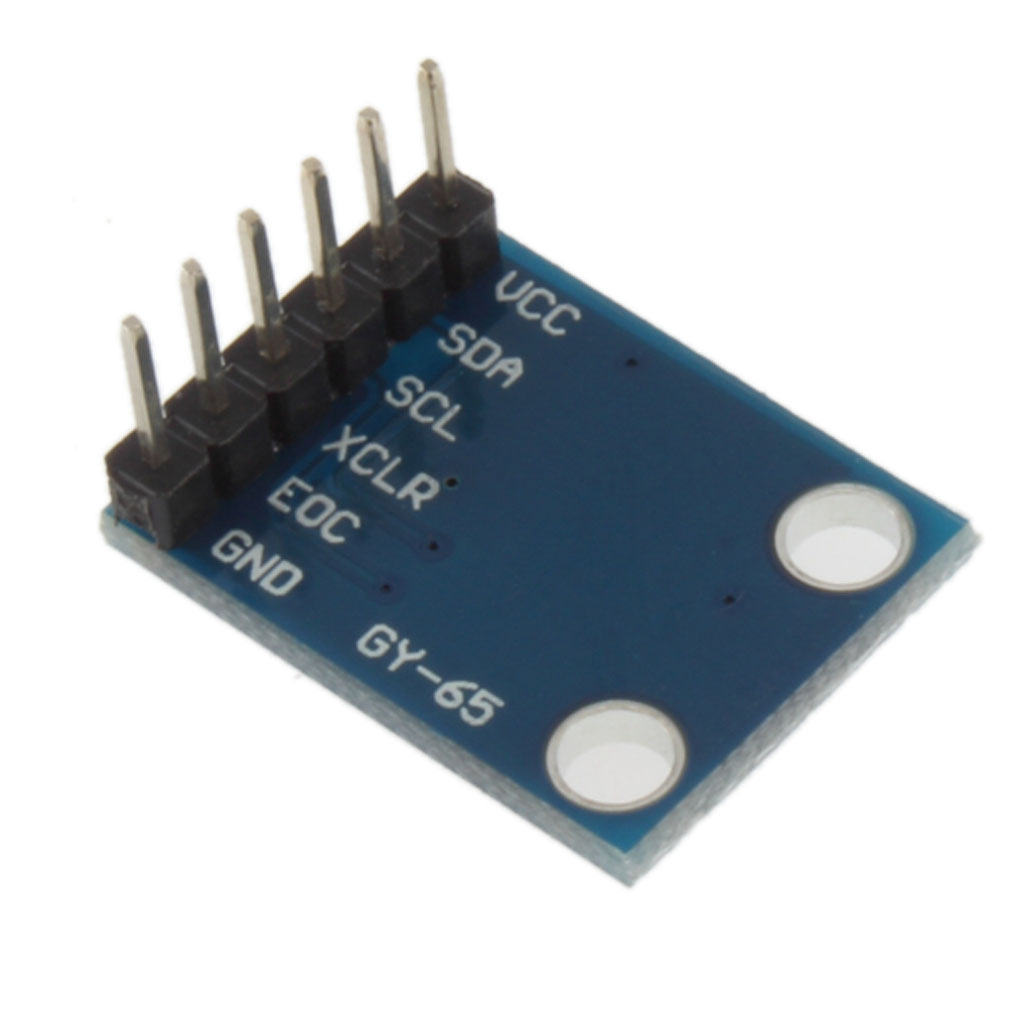
\includegraphics[scale=0.85]{bmp085_gora}
\caption{Czujnik ciśnienia BMP085 - widok z góry}
\label{fig:bmp085_gora}
\end{figure}

Pomiar temperatury oraz ciśnienia jest kompensowany przy użyciu danych kalibracyjnych, które przechowywane są w pamięci EEPROM czujnika.

\section*{Pobieranie danych z czujnika}
BMP085 jest przystosowany do łączności za pomocą magistrali $I^2C$. Wymaga on do poprawnego działania czterach przewodów: zasilania, uziemienia, linii danych SDA oraz linii zegara SCL. Linie SCL oraz SDA wymagają podpięcia rezystora podciągającego do zasilania o oporze 4,7~$k\Omega$. Zastosowany w pracy czujnik jest zbudowany na gotowej płytce drukowanej z podpiętymi już rezystorami podciągającymi, dzięki temu jest on gotowy do podpięcia kablami, bez dodatkowego montowania układu.

Czujnik podpięty do magistrali $I^2C$ otrzymuje adres, pod którym on się znajduje w strukturze. BMP085 domyślnie posiada adres 0x68 i przy użyciu tego adresu można odczytywać oraz zapisywać do niego dane.

\begin{figure}[h]
\centering
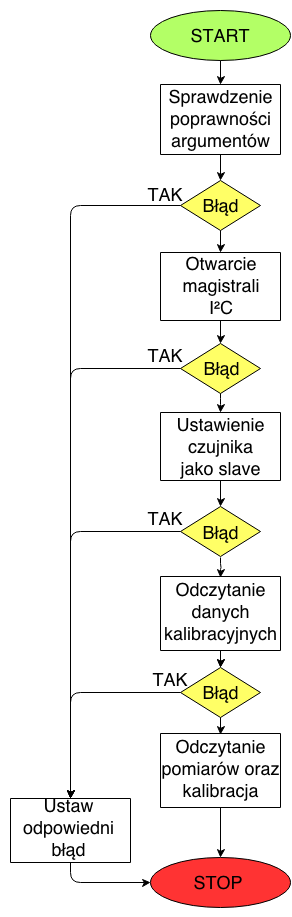
\includegraphics[scale=0.6]{diagram_bmp085}
\caption{Diagram odczytu danych z czujnika BMP085}
\label{fig:diagram_bmp085}
\end{figure}